\chapter{Processes}

\epigraph{Who needs process isolation?}{Intel Marketing on Meltdown and Spectre}

In the beginning, there is a kernel. The operating system kernel is a special piece of software. This is the piece of software that is loaded up before all of your other programs even consider getting booted up. What the kernel does is the following, abbreviated

\begin{enumerate}
  \def\labelenumi{\arabic{enumi}.}
  \tightlist
\item
  The operating system executes ROM or read only code
\item
  The operating system then executes a \keyword{boot\_loader} or \keyword{EFI} extensions nowadays
\item
  The boot\_loader loads your kernels
\item
  Your kernel executes \keyword{init} to \href{https://en.wikipedia.org/wiki/Bootstrapping}{bootstrap} itself from nothing
\item
  The kernel executes startup scripts
\item
  The kernel executes userland scripts, and you get to use your computer!
\end{enumerate}

You don't need to know the specifics of the booting process, but there it is.
When you are executing in user space the kernel provides some important operations that programs don't have to worry about. 

\begin{itemize}
\item Scheduling Processes and threads
\item Handling synchronization primitives 
\item Providing System Calls like \keyword{write} or \keyword{read} 
\item Manages virtual memory and low level binary devices like \keyword{usb} drivers 
\item Handles reading and understanding a filesystem 
\item Handles communicating over networks 
\item Handles communications with other processes 
\item Dynamically linking libraries
\end{itemize}

The kernel handles all of this stuff in kernel mode.
Kernel mode gets you greater power, like executing extra CPU instructions but at the cost of one failure crashes your entire computer -- ouch.
That is what you are going to interacting with in this class.
One of the things that you have already become familiar with is that the kernel gives you file descriptors when you open text files.
Here is a zine from Julia Evans that details it a bit.

\begin{figure}[htbp]
  \centering
  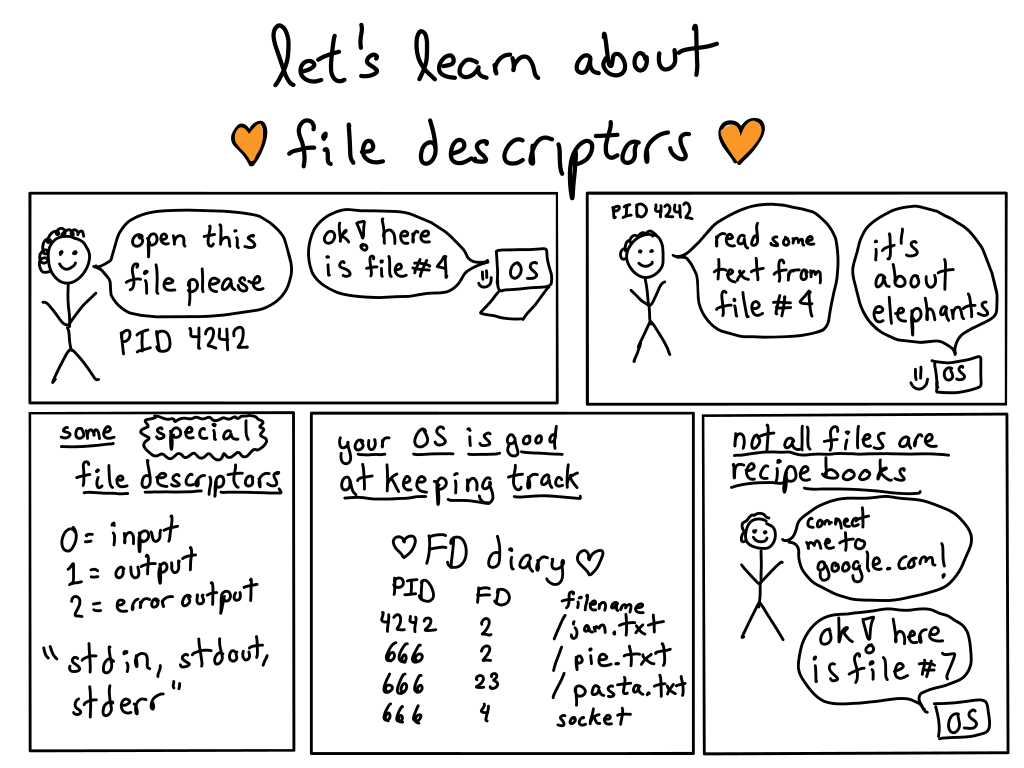
\includegraphics[width=.8\textwidth]{processes/images/file-descriptors.png}
  \caption{File Descriptors}
\end{figure}

As the little zine shows, the Kernel keeps track of the file descriptors and what they point to.
We will see later that file descriptors need not point to actual files and the OS keeps track of them for you.
Also, notice that between processes file descriptors may be reused but inside of a process they are unique.
File descriptors also have a notion of position. You can read a file on disk completely because the OS keeps track of the position in the file, and that belongs to your process as well.

\section{Processes}

A process an instance of a computer program that may be running.
Processes have a lot of things at their disposal.
At the start of each program you get one process, but each program can make more processes.
In fact, your operating system starts up with only one process and all other processes are forked off of that -- all of that is done under the hood when booting up. A program consists of the following.

\begin{itemize}
\item A binary format: This tells the operating system which set of bits in the binary are what -- which part is executable, which parts are constants, which libraries to include etc. 
\item A set of machine instructions 
\item A number denoting which instruction to start from
\item Constants
\item Libraries to link and where to fill in the address of those libraries
\end{itemize}

When your operating system starts on a linux machine, there is a process called \keyword{init.d} that gets created.
That process is a special one handling signals, interrupts, and a persistence module for certain kernel elements.
Whenever you want to make a new process, you call \keyword{fork} and use \keyword{exec} to load another program.

Processes are very powerful but they are isolated!
That means that by default, no process can communicate with another process.
This is very important because if you have a large system (let's say the University of Illinois Engineering Workstations) then you want some processes to have higher privileges than your average user, and one certainly doesn't want the average user to be able to bring down the entire system either on purpose or accidentally by modifying a process.

\begin{lstlisting}[language=C]
int secrets;
secrets++;
printf("%d\n", secrets);
\end{lstlisting}

On two different terminals, as you would guess they would both print out 1 not 2.
Even if we changed the code to do something really hacky, there would be no way to change another process' state.
Okay, check out the Post-Mortems chapter if you want to break some things).

\section{Process Contents}

\subsection{Memory Layout}

When a process starts, it gets its own address space. Each process gets the following.
\begin{itemize}
\item \textbf{A Stack}.
The stack is the place where automatic variable and function call return addresses are stored.
Every time a new variable is declared, the program moves the stack pointer down to reserve space for the variable.
This segment of the stack is Writable but not executable.
If the stack grows too far -- meaning that it either grows beyond a preset boundary or intersects the heap -- you will get a stackoverflow most likely resulting in a SEGFAULT.
\textbf{The stack is statically allocated by default meaning that there is only a certain amount of space to which one can write} 

\item \textbf{A Heap}.
The heap is an expanding region of memory.
If you want to allocate a large object, it goes here.
The heap starts at the top of the text segment and grows upward, meaning sometimes when you call \keyword{malloc} that it asks the operating system to push the heap boundary upward.
More on that in the memory allocation chapter.
This area is also writable but not executable.
One can run out of heap memory if the system is constrained or if you run out of addresses. This is more common on a 32bit system. 

\item \textbf{A Data Segment} This contains all of your globals.
This section starts at the end of the text segment and is static in size because the amount of globals is known at compile time.
There are two areas to the data usually the \textbf{IBSS} and the \textbf{UBSS} which stand for the initialized basic service set and the uninitialized data segment respectively.
This section is writable but not executable. 

\item \textbf{A Text Segment}.
This is where all your code is stored -- all the 1's and 0's.
The program counter moves through this segment executing instructions and moving down the next instruction.
It is important to note that this is the only executable section of the code created by default.
If you try to change the code while it's running, most likely you will segfauls.
There are ways around it, but we won't be exploring those in this course.
Why doesn't it start at zero? Because of \href{https://en.wikipedia.org/wiki/Address_space_layout_randomization}{Address Space Layout Randomization}. It is outside the scope of this class but know that it exists.
\end{itemize}

\subsection{Other Contents}

To keep track of all these processes, your operating system gives each process a number and that process is called the PID, process ID.
Processes also have a \keyword{ppid} which is short for parent process id.
Every process has a parent, that parent could be \keyword{init.d}.

Processes could also contain 

\begin{itemize}
\item Running State - Whether a process is getting ready, running, stopped, terminated etc. 
\item File Descriptors - List of mappings from integers to real devices (files, usb sticks, sockets) 
\item Permissions - What \keyword{user} the file is running on and what \keyword{group} the process belongs to. The process can then only do this admissible to the \keyword{user} or \keyword{group} like opening a file that the \keyword{user} has made exclusives. There are tricks to make a program not be the user who started the program i.e. \keyword{sudo} takes a program that a \keyword{user} starts and executes it as \keyword{root}. 
\item Arguments - a list of strings that tell your program what parameters to run under
\item Environment List - a list of strings in the form \keyword{NAME=VALUE} that one can modify.
\end{itemize}

\section{Intro to Fork}

\subsection{A word of warning}

Process forking is a powerful and dangerous tool.
If you mess up and cause a fork bomb, \textbf{you can bring down the entire system}.
To reduce the chances of this, limit your maximum number of processes to a small number e.g 40 by typing \keyword{ulimit\ -u\ 40} into a command line.
Note, this limit is only for the user, which means if you fork bomb, then you won't be able to kill all of the processes you just created since calling \keyword{killall} requires your shell to \keyword{fork()} \ldots{} ironic right? One solution is to spawn another shell instance as another user (for example root) before hand and kill processes from there.
Another is to use the built in \keyword{exec} command to kill all the user processes (careful you only have one shot at this).
Finally you could reboot the system, but you only have one shot at this with the exec function.
When testing fork() code, ensure that you have either root and/or physical access to the machine involved.
If you must work on fork() code remotely, remember that \textbf{kill -9 -1} will save you in the event of an emergency.

TL;DR: Fork can be \textbf{extremely} dangerous if you aren't prepared for it. \textbf{You have been warned.}

\subsection{What does fork do?}

The \keyword{fork} system call clones the current process to create a new process.
It creates a new process (the child process) by duplicating the state of the existing process with a few minor differences.
The child process does not start from main.
Instead it executes the next line after the \keyword{fork()} just as the parent process does.
Just as a side remark, in older UNIX systems, the entire address space of the parent process was directly copied (regardless of whether the resource was modified or not).
These days, kernel performs \href{https://en.wikipedia.org/wiki/Copy-on-write}{copy-on-write}, which saves a lot of resources, while being very time efficient.
Here's a very simple example

\begin{lstlisting}[language=C]
  printf("I'm printed once!\n");
  fork();
  // Now there are two processes running if fork succeeded
  // and each process will print out the next line.
  printf("You see this line twice!\n");
\end{lstlisting}

The following program may print out 42 twice - but the \keyword{fork()} is after the \keyword{printf}!? Why?

\begin{lstlisting}[language=C]
  #include <unistd.h> /*fork declared here*/
  #include <stdio.h> /* printf declared here*/
  int main() {
    int answer = 84 >> 1;
    printf("Answer: %d", answer);
    fork();
    return 0;
  }
\end{lstlisting}

The \keyword{printf} line \emph{is} executed only once however notice that the printed contents is not flushed to standard out. There's no newline printed, we didn't call \keyword{fflush}, or change the buffering mode. The output text is therefore still in process memory waiting to be sent. When \keyword{fork()} is executed the entire process memory is duplicated including the buffer. Thus the child process starts with a non-empty output buffer which will be flushed when the program exits.

To write code that is different for the parent and child process, check the return value of \keyword{fork()}.
If fork() returns -1, that implies something went wrong in the process of creating a new child.
One should check the value stored in \emph{errno} to determine what kind of error occurred; commons one include EAGAIN and ENOMEM Which are essentially try again and out of memory.
Similarly, a return value of 0 indicates that we are in the child process, while a positive integer shows that we are in parent process.
The positive value returned by \keyword{fork()} gives as the process id (\emph{pid}) of the child.

Another way to remember which is which is that the child process can find its parent - the original process that was duplicated - by calling \keyword{getppid()} - so does not need any additional return information from \keyword{fork()}.
The parent process however can only find out the id of the new child process from the return value of \keyword{fork}:

\begin{lstlisting}[language=C]
  pid_t id = fork();
  if (id == -1) exit(1); // fork failed 
  if (id > 0) { 
    // I'm the original parent and 
    // I just created a child process with id 'id'
    // Use waitpid to wait for the child to finish
  } else { // returned zero
    // I must be the newly made child process
  }
\end{lstlisting}

A slightly silly example is shown below. What will it print? Try it with multiple arguments to your program.

\begin{lstlisting}[language=C]
  #include <unistd.h>
  #include <stdio.h>
  int main(int argc, char **argv) {
    pid_t id;
    int status; 
    while (--argc && (id=fork())) {
      waitpid(id,&status,0); /* Wait for child*/
    }
    printf("%d:%s\n", argc, argv[argc]);
    return 0;
  }
\end{lstlisting}

Another example is below. This is the amazing parallel apparent-O(N) \emph{sleepsort} is today's silly winner. First published on \href{https://dis.4chan.org/read/prog/1295544154}{4chan in 2011}. A version of this awful but amusing sorting algorithm is shown below.

\begin{lstlisting}[language=C]
  int main(int c, char **v) {
    while (--c > 1 && !fork());
    int val  = atoi(v[c]);
    sleep(val);
    printf("%d\n", val);
    return 0;
  }
\end{lstlisting}

Note: The algorithm isn't actually O(N) because of how the system scheduler works, though you can get faster times.

\subsection{What is a fork bomb?}

A `fork bomb' is when you attempt to create an infinite number of processes.
This will often bring a system to a near-standstill as it attempts to allocate CPU time and memory to a very large number of processes that are ready to run.
System administrators don't like fork-bombs and may set upper limits on the number of processes each user can have or may revoke login rights because it creates a disturbance in the force for other users' programs.
You can also limit the number of child processes created by using \keyword{setrlimit()}.
fork bombs are not necessarily malicious - they occasionally occur due to student coding errors.
Below is a simple example.

\begin{lstlisting}[language=C]
  while (1) fork();
\end{lstlisting}

There may even be subtle forkbombs that occur when you are being careless while coding.

\begin{lstlisting}[language=C]
  #include <unistd.h>
  #define HELLO_NUMBER 10

  int main(){
    pid_t children[HELLO_NUMBER];
    int i;
    for(i = 0; i < HELLO_NUMBER; i++){
      pid_t child = fork();
      if(child == -1){
        break;
      }
      if(child == 0){ //I am the child
        execlp("ehco", "echo", "hello", NULL);
      }
      else{
        children[i] = child;
      }
    }

    int j;
    for(j = 0; j < i; j++){
      waitpid(children[j], NULL, 0);
    }
    return 0;
  }
\end{lstlisting}

We misspelled \keyword{ehco}, so we can't \keyword{exec} it. What does this mean? Instead of creating 10 processes we just created \textbf{1024 processes, fork bombing our machine. How could we prevent this? Put an exit right after exec so in case exec fails we won't end up fork bombing our machine.}

\subsection{POSIX Fork Detailings}

POSIX determines what the standards of fork are. The commonly expected standards are detailed \href{https://pubs.opengroup.org/onlinepubs/009695399/functions/fork.html}{in the posix fork page} Here are a summary of what gets inherited

\begin{enumerate}
\item Fork will return a non-negative integer on success
\item A child will inherit any open file descriptors of the parent. That means if a parent reads a bit of the file and forks, the child will start at that offset. Any other flags are also carried over.
\item Pending signals are not inherited. This means that if a parent has a pending signal and creates a child, the child will not receive that signal unless another process signals the child.
\item The process will be created with one thread (more on that later, the general consensus is to not fork and pthread at the same time).
\item Since we have copy on write, read-only memory addresses are shared between processes
\item If you set up certain regions of memory, they are shared between processes.
\item Signal handlers are inherited but can be changed
\item Current working directory is inherited but can be changed
\item Environment variables are inherited but can be changed
\end{enumerate}

Key differences include: 
\begin{itemize}
\item The process id returned by \keyword{getpid()}. The parent process id returned by \keyword{getppid()}. 
\item The parent is notified via a signal, SIGCHLD, when the child process finishes but not vice versa. 
\item The child does not inherit pending signals or timer alarms. For a complete list see the \href{http://man7.org/linux/man-pages/man2/fork.2.html}{fork man page}
\item The child has its own set of environment variables
\end{itemize}

\section{Waiting and Execing}

If the parent process wants waits for the child to finish, \keyword{waitpid} (or \keyword{wait}).

\begin{lstlisting}[language=C]
  pid_t child_id = fork();
  if (child_id == -1) { perror("fork"); exit(EXIT_FAILURE);}
  if (child_id > 0) { 
    // We have a child! Get their exit code
    int status; 
    waitpid( child_id, &status, 0 );
    // code not shown to get exit status from child
  } else { // In child ...
    // start calculation
    exit(123);
  }
\end{lstlisting}

\keyword{wait} is a simpler version of \keyword{waitpid}.
\keyword{wait} accepts a pointer to an integer and waits on any child process.
After the first one changes state \keyword{wait} returns.
\keyword{waitpid} is similar to \keyword{wait} but it has a few differences.
First, you \textit{can} wait on a specific process, or you can pass in special values for the \keyword{pid} to do different things (check the man pages).
The last parameter to waitpid is an option parameter. The options are listed below


\begin{enunmerate}
\item WNOHANG - Return whether or not the searched process is exited
\item WNOWAIT - Wait, but leave the child waitable by another wait call
\item WEXITED - Wait for exited children
\item WSTOPPED - Wait for stopped children
\item WCONTINUED - Wait for continued children
\end{enunmerate}

It is generally poor programming practice to use signals in program logic.
Signals have no timeframe of delivery and no assurance that they will be delivered.
If you need to communicate between two processes, there are other ways of doing so.

Exit statuses or the value stored in the integer pointer for both of the calls above are explained below.

\subsection{Exit statuses}

To find the return value of \keyword{main()} or value included in \keyword{exit()}), Use the \texttt{Wait macros} - typically you will use \keyword{WIFEXITED} and \keyword{WEXITSTATUS} . See \keyword{wait}/\keyword{waitpid} man page for more information.

\begin{lstlisting}[language=C][language=C]
  int status;
  pid_t child = fork();
  if (child == -1) return 1; //Failed
  if (child > 0) { /* I am the parent - wait for the child to finish */
    pid_t pid = waitpid(child, &status, 0);
    if (pid != -1 && WIFEXITED(status)) {
      int low8bits = WEXITSTATUS(status);
      printf("Process %d returned %d" , pid, low8bits);
    }
  } else { /* I am the child */
    // do something interesting
    execl("/bin/ls", "/bin/ls", ".", (char *) NULL); // "ls ."
  }
\end{lstlisting}

A process can only have 256 return values, the rest of the bits are informational, this is done by bit shifting.
But, The kernel has an internal way of keeping track of signaled, exited, or stopped.
That API is abstracted so that that the kernel developers are free to change at will.
Remember that these macros only make sense if the precondition is met.
Meaning that a process' exit status won't be defined if the process isn't signaled.
The macros will not do the checking for you, so it's up to the programmer to make sure the logic checks out.
As an example above, you should use the \keyword{WIFSTOPPED} to check if a process was stopped and then the \keyword{WSTOPSIG} to find the signal that stopped it.
As such there is no need to memorize the following, this is just a high level overview of how information is stored inside the status variables. From \keyword{sys/wait.h} of an old Berkeley kernel\cite{sys/wait.h}:

\begin{lstlisting}[language=C][language=C]
  /* If WIFEXITED(STATUS), the low-order 8 bits of the status. */
  #define _WSTATUS(x) (_W_INT(x) & 0177)
  #define _WSTOPPED 0177    /* _WSTATUS if process is stopped */
  #define WIFSTOPPED(x) (_WSTATUS(x) == _WSTOPPED)
  #define WSTOPSIG(x) (_W_INT(x) >> 8)
  #define WIFSIGNALED(x)  (_WSTATUS(x) != _WSTOPPED && _WSTATUS(x) != 0)
  #define WTERMSIG(x) (_WSTATUS(x))
  #define WIFEXITED(x)  (_WSTATUS(x) == 0)
\end{lstlisting}

There is an untold convention about exit codes.
If the process exited normally and everything was successful, then a zero should be returned.
Beyond that, there isn't too many conventions except the ones that you place on yourself.
If you know how the program you spawn is going to interact, you may be able to make more sense of the 256 error codes.
You could in fact write your program to return \texttt{1} if the program went to stage 1 (like writing to a file) \texttt{2} if it did something else etc... But none of the unix programs are designed to follow that for simplicity sake.


\subsection{Zombies and Orphans}

It is good practice to wait on your children!
If you don't wait on your children they become zombies.
Zombies occur when a child terminates and then take up a spot in the kernel process table for your process.
The process table keeps information about that process like pid, status, how it was killed.
The only way to get rid of a zombie is to wait on your children.
If you never wait on your children, and the program is long running then you may lose the ability to fork.

You don't always need to wait for your children!
Your parent process can continue to execute code without having to wait for the child process.
If a parent dies without waiting on its children, a process can orphan its children.
Once a parent process completes, any of its children will be assigned to \keyword{init} - the first process with pid of 1.
Thus these children would see \keyword{getppid()} return a value of 1.
These orphans will eventually finish and for a brief moment become a zombie.
The init process automatically waits for all of its children, thus removing these zombies from the system.

\subsection{Extra: How can I asynchronously wait for my child using SIGCHLD?}

Warning: This section uses signals which we have not yet fully introduced. The parent gets the signal SIGCHLD when a child completes, so the signal handler can wait on the process. A slightly simplified version is shown below.

\begin{lstlisting}[language=C]
  pid_t child;

  void cleanup(int signal) {
    int status;
    waitpid(child, &status, 0);
    write(1,"cleanup!\n",9);
  }
  int main() {
    // Register signal handler BEFORE the child can finish
    signal(SIGCHLD, cleanup); // or better - sigaction
    child = fork();
    if (child == -1) { exit(EXIT_FAILURE);}

    if (child == 0) { /* I am the child!*/
      // Do background stuff e.g. call exec   
    } else { /* I'm the parent! */
      sleep(4); // so we can see the cleanup
      puts("Parent is done");
    }
    return 0;
  } 
\end{lstlisting}

The above example however misses a couple of subtle points.
\begin{enumerate}
\item More than one child may have finished but the parent will only get one SIGCHLD signal (signals are not queued)
\item SIGCHLD signals can be sent for other reasons (e.g.~a child process is temporarily stopped)
\item It uses the deprecated \keyword{signal} code
\end{enumerate}

A more robust code to reap zombies is shown below.

\begin{lstlisting}[language=C]
  void cleanup(int signal) {
    int status;
    while (waitpid((pid_t) (-1), 0, WNOHANG) > 0) {

    }
  }
\end{lstlisting}

\section{exec}

To make the child process execute another program, use one of the \href{http://man7.org/linux/man-pages/man3/exec.3.html}{\keyword{exec}} functions after forking.
The \keyword{exec} set of functions replaces the process image with the the process image of what is being called.
This means that any lines of code after the \keyword{exec} call are replaced.
Any other work you want the child process to do should be done before the \keyword{exec} call.
The \href{https://en.wikipedia.org/wiki/Exec_(system_call)\#C_language_prototypes}{Wikipedia article} does a great job helping you make sense of the names of the exec family.
The naming schemes can be shortened mnemonically.

\begin{enumerate}
\item e -- An array of pointers to environment variables is explicitly passed to the new process image.
\item l -- Command-line arguments are passed individually (a list) to the function.
\item p -- Uses the PATH environment variable to find the file named in the file argument to be executed.
\item v -- Command-line arguments are passed to the function as an array (vector) of pointers.
\end{enumerate}

An example of this code is below. This code executes \keyword{ls}

\begin{lstlisting}[language=C]
  #include <unistd.h>
  #include <sys/types.h> 
  #include <sys/wait.h>
  #include <stdlib.h>
  #include <stdio.h>

  int main(int argc, char**argv) {
    pid_t child = fork();
    if (child == -1) return EXIT_FAILURE;
    if (child) { /* I have a child! */
      int status;
      waitpid(child , &status ,0);
      return EXIT_SUCCESS;

    } else { /* I am the child */
      // Other versions of exec pass in arguments as arrays
      // Remember first arg is the program name
      // Last arg must be a char pointer to NULL

      execl("/bin/ls", "/bin/ls","-alh", (char *) NULL);

      // If we get to this line, something went wrong!
      perror("exec failed!");
    }
  }
\end{lstlisting}

Try to decode the following example

\begin{lstlisting}[language=C]
  #include <unistd.h>
  #include <fcntl.h> // O_CREAT, O_APPEND etc. defined here

  int main() {
    close(1); // close standard out
    open("log.txt", O_RDWR | O_CREAT | O_APPEND, S_IRUSR | S_IWUSR);
    puts("Captain's log");
    chdir("/usr/include");
    // execl( executable,  arguments for executable including program name and NULL at the end)

    execl("/bin/ls", /* Remaining items sent to ls*/ "/bin/ls", ".", (char *) NULL); // "ls ."
    perror("exec failed");
    return 0; // Not expected
  }
\end{lstlisting}

There's no error checking in the above code (we assume close,open,chdir etc works as expected). 

\begin{enumerate}
\item \keyword{open} -- will use the lowest available file descriptor (i.e.~1) ; so standard out now goes to the log file. 
\item \keyword{chdir} -- Change the current directory to /usr/include 
\item \keyword{execl} -- Replace the program image with /bin/ls and call its main() method 
\item \keyword{perror} -- We don't expect to get here - if we did then exec failed.
\end{enumerate}

\subsection{Deeper Semantics}

\href{https://pubs.opengroup.org/onlinepubs/009695399/functions/exec.html}{Here is the full POSIX standard for Exec}
What you need to know is the following bullet points (in addition to above).

\begin{enumerate}
\item File descriptors are preserved after an exec. That means if you open a file, and you forget to close it, it remains open in the child.
This is a problem because usually the child doesn't know about those file descriptors and they take up a slot in the file descriptor table and could possible prevent other processes from accessing the file. The one exception to this is if the file descriptor has the Close Exec flag set (more on how to set that later).
\item Various signal semantics (don't need to worry about this yet). If you are coming back to do a re-read, exec'ed processes preserve the signal mask and the pending signal set.
\end{enumerate}

\subsection{Shortcuts}

\keyword{system} pre-packs the above code. Here is how to use it:

\begin{lstlisting}[language=C]

  #include <unistd.h>
  #include <stdlib.h>

  int main(int argc, char**argv) {
    system("ls"); // execl("/bin/sh", "/bin/sh", "-c", "\\"ls\\"")
    return 0;
  }
\end{lstlisting}

The \keyword{system} call will fork, execute the command passed by parameter and the original parent process will wait for this to finish.
This also means that \keyword{system} is a blocking call: The parent process can't continue until the process started by \keyword{system} exits.
Also, \keyword{system} actually creates a shell which is then given the string, which is more overhead than just using \keyword{exec} directly.
The standard shell will use the \keyword{PATH} environment variable to search for a filename that matches the command. Using system will usually be sufficient for many simple run-this-command problems but can quickly become limiting for more complex or subtle problems, and it hides the mechanics of the fork-exec-wait pattern so we encourage you to learn and use \keyword{fork} \keyword{exec} and \keyword{waitpid} instead.
Not only that, it tends to be a huge security risk. By allowing someone to access a shell version of the environment, you can reach all sorts of problems

\begin{lstlisting}[language=C]
  int main(int argc, char**argv) {
    char *to_exec = asprintf("ls %s", argv[1]); 
    system(to_exec);
  }
\end{lstlisting}

Passing something along the lines of argv[1] = "; sudo su" could cause all sorts of problems.

\section{The fork-exec-wait Pattern}

A common programming pattern is to call \keyword{fork} followed by \keyword{exec} and \keyword{wait}.
The original process calls fork, which creates a child process.
The child process then uses exec to start execution of a new program.
Meanwhile the parent uses \keyword{wait} (or \keyword{waitpid}) to wait for the child process to finish. 

\begin{lstlisting}[language=C][language=C]
  #include <unistd.h>

  int main() {
    pid_t pid = fork();
    if (pid < 0) { // fork failure
      exit(1);
    } else if (pid > 0) { // I am the parent
      int status;
      waitpid(pid, &status, 0);
    } else { // I am the child
      execl("/bin/ls", "/bin/ls", NULL);
      exit(1);
    }
  }
\end{lstlisting}

\subsection{Environment Variables}

Environment variables are variables that the system keeps for all processes to use.
Your system has these set up right now!
In Bash, you can check some of these

\begin{lstlisting}[language=C]
  $ echo $HOME
  /home/bhuvy
  $ echo $PATH
  /usr/local/sbin:/usr/bin:...
\end{lstlisting}

How would you get these in C/C++? You can use the \keyword{getenv} and \keyword{setenv} function

\begin{lstlisting}[language=C]
  char* home = getenv("HOME"); // Will return /home/bhuvy
  setenv("HOME", "/home/bhuvan", 1 /*set overwrite to true*/ );
\end{lstlisting}

Environment variables are important because they are inherited between processes and can be used the specify \href{https://pubs.opengroup.org/onlinepubs/9699919799/basedefs/V1_chap08.html}{A standard set of behaviors}
Another security related concern is that environment variables cannot be read by an outside process whereas argv can be.

\section{Further Reading}

Read the man pages! 
\begin{itemize}
\item \href{http://man7.org/linux/man-pages/man2/fork.2.html}{fork} 
\item \href{http://man7.org/linux/man-pages/man3/exec.3.html}{exec} 
\item \href{http://man7.org/linux/man-pages/man2/wait.2.html}{wait}
\end{itemize}

\subsection{Topics}

\begin{itemize}
  \tightlist
\item
  Correct use of fork, exec and waitpid
\item
  Using exec with a path
\item
  Understanding what fork and exec and waitpid do. E.g. how to use their return values.
\item
  SIGKILL vs SIGSTOP vs SIGINT.
\item
  What signal is sent when you press CTRL-C
\item
  Using kill from the shell or the kill POSIX call.
\item
  Process memory isolation.
\item
  Process memory layout (where is the heap, stack etc; invalid memory addresses).
\item
  What is a fork bomb, zombie and orphan? How to create/remove them.
\item
  getpid vs getppid
\item
  How to use the WAIT exit status macros WIFEXITED etc.
\end{itemize}

\section{Questions/Exercises}

\begin{itemize}
\item
  What is the difference between execs with a p and without a p? What does the operating system
\item
  How do you pass in command line arguments to \keyword{execl*}? How about \keyword{execv*}? What should be the first command line argument by convention?
\item
  How do you know if \keyword{exec} or \keyword{fork} failed?
\item
  What is the \keyword{int\ *status} pointer passed into wait? When does wait fail?
\item
  What are some differences between \keyword{SIGKILL}, \keyword{SIGSTOP}, \keyword{SIGCONT}, \keyword{SIGINT}? What are the default behaviors? Which ones can you set up a signal handler for?
\item
  What signal is sent when you press \keyword{CTRL-C}?
\item
  My terminal is anchored to PID = 1337 and has just become unresponsive. Write me the terminal command and the C code to send \keyword{SIGQUIT} to it.
\item
  Can one process alter another processes memory through normal means? Why?
\item
  Where is the heap, stack, data, and text segment? Which segments can you write to? What are invalid memory addresses?
\item
  Code me up a fork bomb in C (please don't run it).
\item
  What is an orphan? How does it become a zombie? How do I be a good parent?
\item
  Don't you hate it when your parents tell you that you can't do something? Write me a program that sends \keyword{SIGSTOP} to your parent.
\item
  Write a function that fork exec waits an executable, and using the wait macros tells me if the process exited normally or if it was signaled. If the process exited normally, then print that with the return value. If not, then print the signal number that caused the process to terminate.
\end{itemize}

\bibliographystyle{plainnat}
\bibliography{processes/processes}
